\documentclass[tikz,border=8pt]{standalone}
% Shared look for every TikZ diagram. Load with \input{../../tools/tikz-style.tex}
\usepackage[T1]{fontenc}
\usepackage{lmodern}
\renewcommand{\sfdefault}{lmr}  % diagrams use the same serif as the text
\usetikzlibrary{arrows.meta, positioning, shapes.geometric, calc, fit, backgrounds}
\definecolor{cblue}{HTML}{4C78A8}
\definecolor{corange}{HTML}{F58518}
\definecolor{cgreen}{HTML}{54A24B}
\definecolor{cred}{HTML}{E45756}
\definecolor{cpurple}{HTML}{B279A2}
\definecolor{cgrey}{HTML}{6B6B6B}
\tikzset{
  every picture/.style={font=\sffamily, line width=1.2pt},
  box/.style={draw=#1, fill=#1!12, rounded corners=4pt, align=center, inner sep=7pt, minimum height=1.1cm},
  box/.default=cgrey,
  arrow/.style={-{Stealth[length=3mm]}, draw=cgrey, line width=1.4pt},
  title/.style={font=\sffamily\bfseries\Large},
  note/.style={font=\sffamily\small, text=cgrey, align=center},
}
\AtBeginDocument{\hyphenpenalty=10000 \exhyphenpenalty=10000}

% Overview: the hallway of the chapter, 10 cells of 1 m in a loop, doors at cells 1, 3 and 7. The robot's door
% sensor says "door". Three cells fit the reading, so the robot keeps all three, each with probability 1/3.
\begin{document}
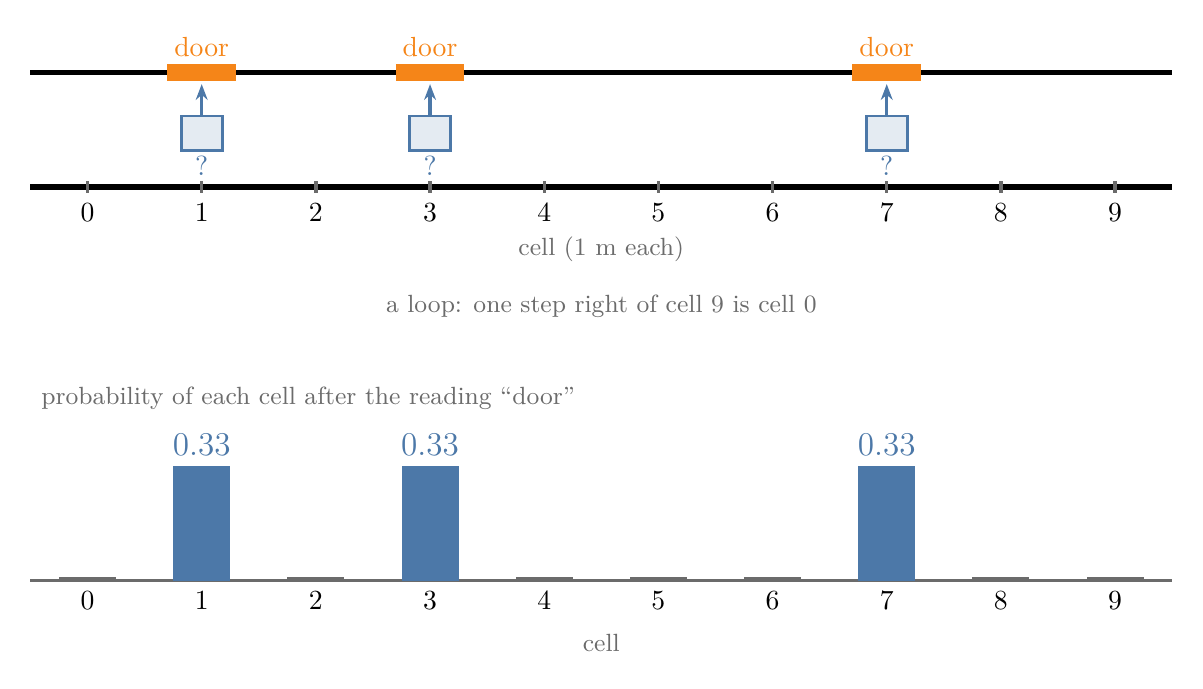
\begin{tikzpicture}[x=1.45cm, y=1.45cm, every node/.append style={font=\large}]
  % walls
  \draw[black, line width=2pt] (-0.5,1) -- (9.5,1);
  \draw[black, line width=2pt] (-0.5,0) -- (9.5,0);
  \foreach \d in {1,3,7} {
    \draw[corange, line width=6pt] (\d-0.3,1.0) -- (\d+0.3,1.0);
    \node[corange, above, font=\normalsize] at (\d,1.05) {door};
  }
  % ghost robots at the doors
  \foreach \d in {1,3,7} {
    \draw[cblue, fill=cblue!15, line width=1pt] (\d-0.18,0.32) rectangle (\d+0.18,0.62);
    \draw[-{Stealth[length=2mm]}, cblue] (\d,0.62) -- (\d,0.9);
    \node[cblue, font=\normalsize] at (\d,0.18) {?};
  }
  % metre ticks
  \foreach \t in {0,...,9} { \draw[cgrey] (\t,-0.05) -- (\t,0.05); \node[below, font=\normalsize] at (\t,-0.05) {\t}; }
  \node[note] at (4.5,-0.55) {cell (1 m each)};
  \node[note, cgrey] at (4.5,-1.05) {a loop: one step right of cell 9 is cell 0};
  % belief bars
  \begin{scope}[yshift=-5.0cm]
    \draw[cgrey, line width=1pt] (-0.5,0) -- (9.5,0);
    \foreach \t in {0,...,9} \node[below, font=\normalsize] at (\t,0) {\t};
    \foreach \t in {0,2,4,5,6,8,9} \fill[cgrey] (\t-0.25,0) rectangle (\t+0.25,0.03);
    \foreach \d in {1,3,7} { \fill[cblue] (\d-0.25,0) rectangle (\d+0.25,1.0); \node[above, cblue] at (\d,1.0) {0.33}; }
    \node[note, anchor=west] at (-0.5,1.6) {probability of each cell after the reading ``door''};
    \node[note] at (4.5,-0.55) {cell};
  \end{scope}
\end{tikzpicture}
\end{document}
